% No-GPS Drone Project --- Technical Report
% Compile with: pdflatex project_report.tex  (run twice for references)
\documentclass[11pt,a4paper]{article}

% ── Packages ──────────────────────────────────────────────────────────────────
\usepackage[T1]{fontenc}
\usepackage[utf8]{inputenc}
\usepackage[margin=2.5cm]{geometry}
\usepackage{lmodern}
\usepackage{microtype}
\usepackage{graphicx}
\usepackage{xcolor}
\usepackage{booktabs}
\usepackage{longtable}
\usepackage{enumitem}
\usepackage{listings}
\usepackage{tikz}
\usepackage{hyperref}
\usepackage{amsmath}
\usepackage{array}
\usepackage{caption}
\usepackage{subcaption}
\usepackage{titlesec}
\usepackage{fancyhdr}
\usepackage{mdframed}

\usetikzlibrary{arrows.meta, positioning, shapes.geometric, fit, backgrounds,
                decorations.pathreplacing, calc}

% ── Colours ───────────────────────────────────────────────────────────────────
\definecolor{simblue}{RGB}{30,100,200}
\definecolor{locgreen}{RGB}{30,160,80}
\definecolor{detred}{RGB}{200,50,50}
\definecolor{ctrlgold}{RGB}{180,130,0}
\definecolor{ardu}{RGB}{100,60,180}
\definecolor{codebg}{RGB}{245,245,245}
\definecolor{linkblue}{RGB}{20,80,160}

% ── Hyperref ──────────────────────────────────────────────────────────────────
\hypersetup{
  colorlinks=true,
  linkcolor=linkblue,
  urlcolor=linkblue,
  citecolor=linkblue,
  pdftitle={No-GPS Drone Project --- Technical Report},
  pdfauthor={Frank Lin},
}

% ── Header / Footer ───────────────────────────────────────────────────────────
\pagestyle{fancy}
\fancyhf{}
\rhead{\small No-GPS Drone Project}
\lhead{\small Technical Report}
\cfoot{\thepage}
\renewcommand{\headrulewidth}{0.4pt}

% ── Code listings ─────────────────────────────────────────────────────────────
\lstset{
  backgroundcolor=\color{codebg},
  basicstyle=\ttfamily\small,
  breaklines=true,
  frame=single,
  framerule=0.4pt,
  rulecolor=\color{gray!40},
  keywordstyle=\color{simblue}\bfseries,
  commentstyle=\color{gray},
  stringstyle=\color{locgreen},
  numbers=left,
  numberstyle=\tiny\color{gray},
  numbersep=6pt,
  tabsize=4,
  captionpos=b,
}

% ── Section style ─────────────────────────────────────────────────────────────
\titleformat{\section}{\large\bfseries\color{black}}{}{0pt}{}[\titlerule]
\titleformat{\subsection}{\normalsize\bfseries}{}{0pt}{}

% ── Milestone box ─────────────────────────────────────────────────────────────
\newmdenv[
  backgroundcolor=green!8,
  linecolor=green!50!black,
  linewidth=0.6pt,
  roundcorner=3pt,
  innerleftmargin=8pt,
  innerrightmargin=8pt,
  innertopmargin=5pt,
  innerbottommargin=5pt,
]{donebox}

\newmdenv[
  backgroundcolor=orange!10,
  linecolor=orange!70!black,
  linewidth=0.6pt,
  roundcorner=3pt,
  innerleftmargin=8pt,
  innerrightmargin=8pt,
  innertopmargin=5pt,
  innerbottommargin=5pt,
]{todobox}

% ─────────────────────────────────────────────────────────────────────────────
\begin{document}

% ── Title page ────────────────────────────────────────────────────────────────
\begin{titlepage}
  \centering
  \vspace*{2cm}
  {\Huge\bfseries No-GPS Drone Project\par}
  \vspace{0.8cm}
  {\Large\itshape Technical Report\par}
  \vspace{0.4cm}
  {\large GPS-Denied Autonomous UAV Localisation \& Object Detection\par}
  \vspace{2cm}
  \begin{mdframed}[backgroundcolor=gray!10,linecolor=gray!40]
    \centering
    \textbf{Location:} Chiayi, Taiwan \quad $23.4509^\circ$N, $120.2861^\circ$E\\[4pt]
    \textbf{Stack:} Isaac Sim 6.0 \,·\, AnyLoc \,·\, YOLOv8 \,·\, ArduPilot MAVLink\\[4pt]
    \textbf{Competition:} 2nd UAV Defense Challenge (ROC MND) --- GPS-denied multi-target detection
  \end{mdframed}
  \vspace{2cm}
  {\large Frank Lin\par}
  \vspace{0.3cm}
  {\normalsize May 2026\par}
  \vfill
  \textcolor{gray}{\small Validated in NVIDIA Isaac Sim before real-hardware deployment}
\end{titlepage}

% ── Table of contents ─────────────────────────────────────────────────────────
\tableofcontents
\newpage

% ─────────────────────────────────────────────────────────────────────────────
\section{Project Overview}
\label{sec:overview}
% ─────────────────────────────────────────────────────────────────────────────

This project builds a drone system that can \textbf{localise itself and detect objects without GPS},
using visual place recognition (AnyLoc), object detection (YOLOv8), and ArduPilot for flight
control. The full pipeline is validated in NVIDIA Isaac Sim before deployment to real hardware.

\subsection*{Motivation --- Competition Context}

The system is developed for the \textit{2nd UAV Defense Application Challenge}
(2nd National Defense UAV Challenge, ROC) organised by the Republic of China Ministry of National Defense.
The competition theme is \textit{GPS-denied autonomous UAV multi-target reconnaissance}:
a GNSS jammer is physically mounted on the drone, and teams must still autonomously navigate,
identify, and geo-locate targets.

\begin{table}[h]
\centering
\caption{Competition requirements vs.\ project status}
\begin{tabular}{@{}lll@{}}
\toprule
\textbf{Requirement} & \textbf{Project approach} & \textbf{Status}\\
\midrule
GPS-denied navigation & AnyLoc + Visual Odometry & Done\\
Autonomous flight & ArduPilot EKF3 + GUIDED mode & In progress\\
Vehicle detection (cars) & YOLOv8l (VisDrone) & Done\\
Target geo-location & AnyLoc anchor + nadir projection & Done\\
Localisation accuracy ($\leq$50 m) & 15--20 m anchor error & Meets requirement\\
\bottomrule
\end{tabular}
\end{table}

\subsection*{Software Stack}

\begin{itemize}[leftmargin=1.6cm]
  \item[\textbf{Isaac Sim}] NVIDIA Isaac Sim 6.0.0 (Kit 106, Python 3.12) --- physics simulation, Cesium terrain, nadir camera output.
  \item[\textbf{AnyLoc}] Universal visual place recognition --- DINOv2 ViT-B/14 + VLAD + FAISS --- provides GPS-free localisation at 15--20 m accuracy.
  \item[\textbf{YOLOv8}] \texttt{yolov8l\_visdrone.pt} --- YOLOv8-Large pre-trained on VisDrone 2019 DET (10 aerial vehicle classes).
  \item[\textbf{ArduPilot}] Open-source autopilot --- SITL JSON backend connects to Isaac Sim; EKF3 fuses AnyLoc position via \texttt{VISION\_POSITION\_ESTIMATE}.
  \item[\textbf{pymavlink}] MAVLink protocol library --- connects Python control code directly to ArduPilot over TCP.
\end{itemize}

% ─────────────────────────────────────────────────────────────────────────────
\section{System Pipeline}
\label{sec:pipeline}
% ─────────────────────────────────────────────────────────────────────────────

Figure~\ref{fig:pipeline} shows the full data flow from simulation to flight commands.

\begin{figure}[p]
\centering
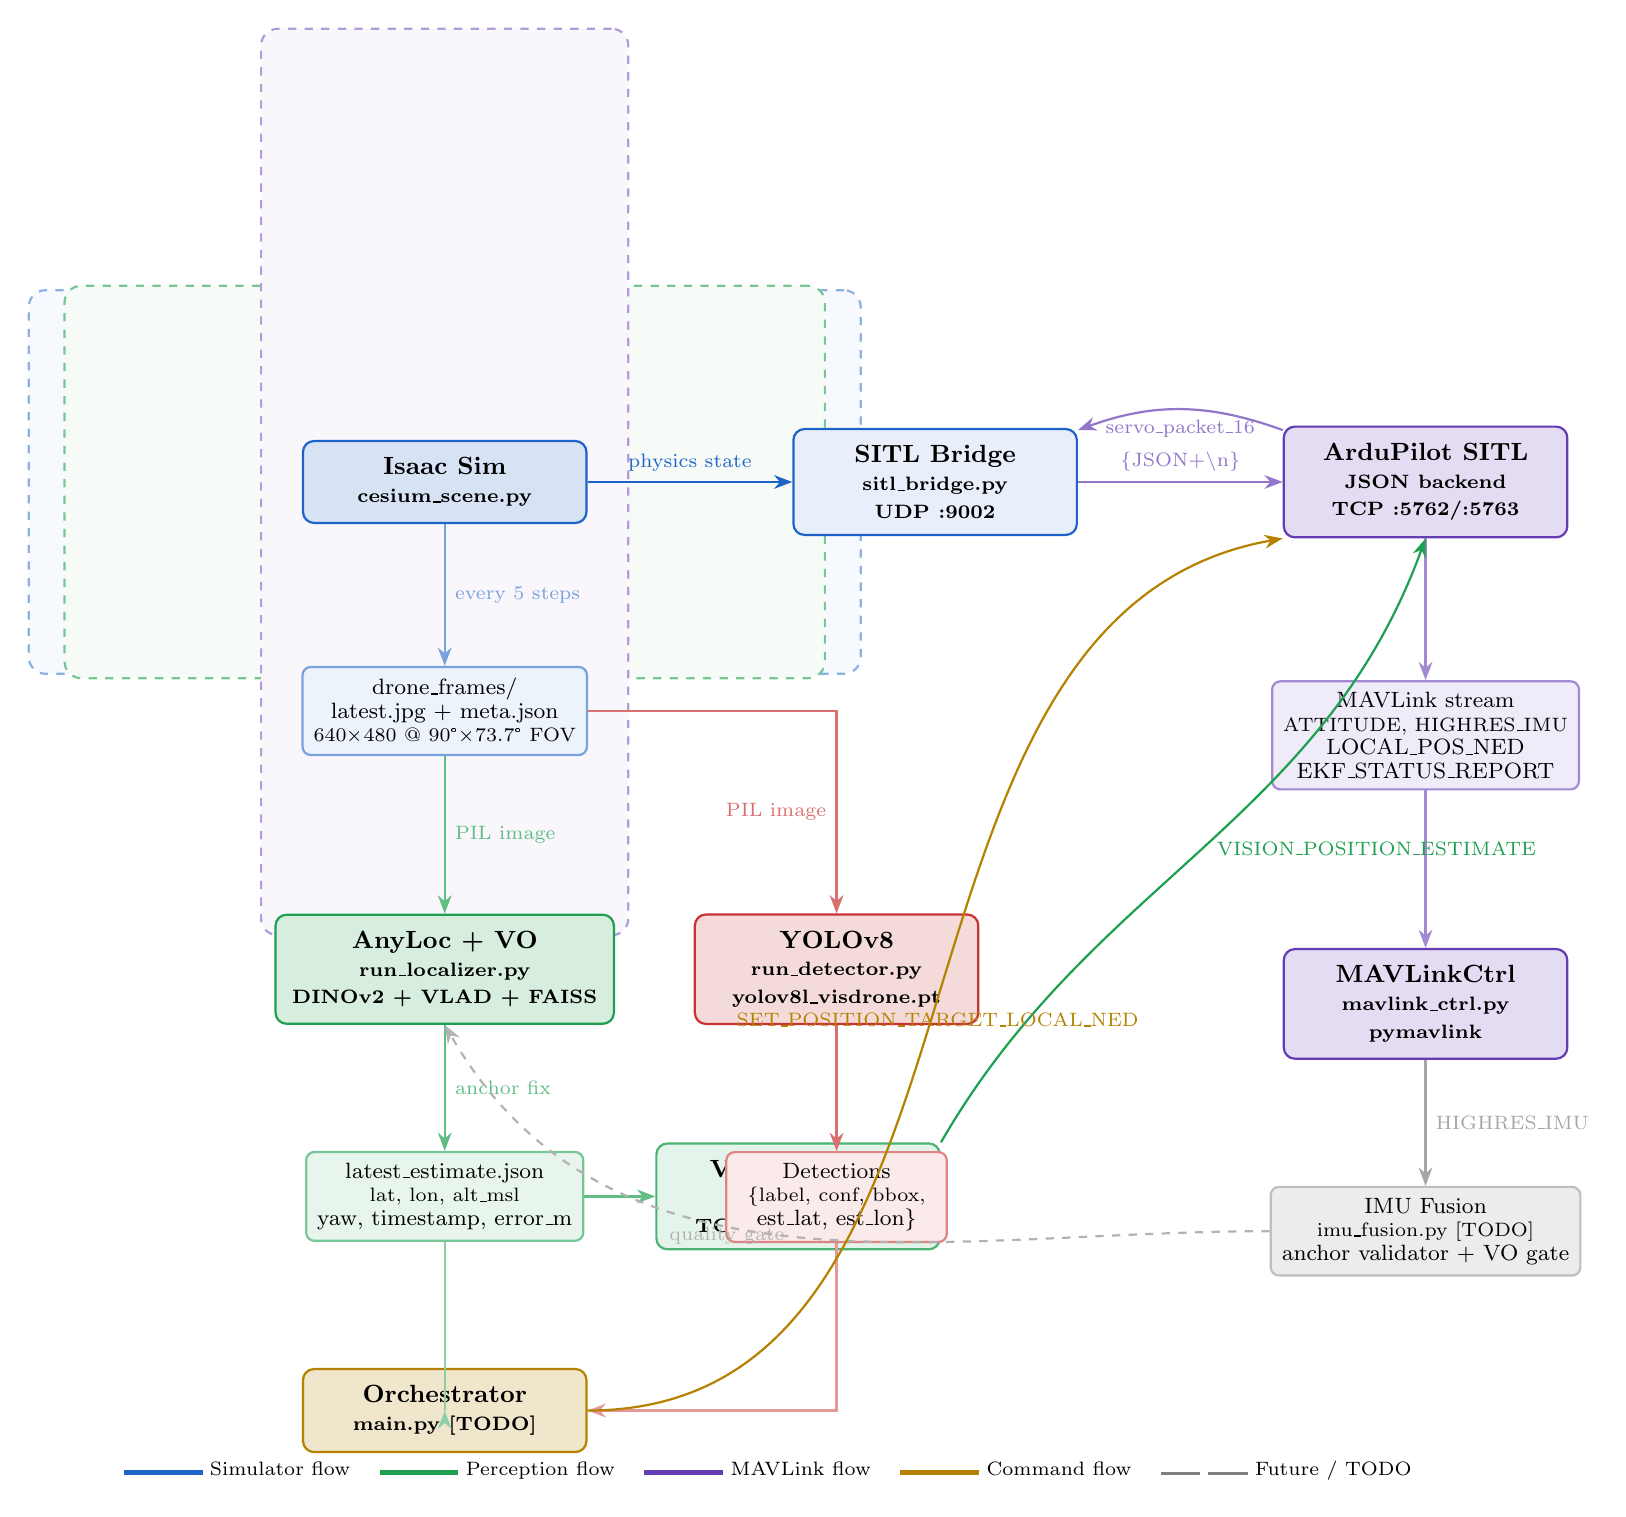
\begin{tikzpicture}[
  >=Stealth,
  node distance=0pt,
  block/.style={
    rectangle, rounded corners=4pt,
    draw, thick,
    minimum width=3.6cm, minimum height=0.9cm,
    align=center, font=\small\bfseries,
    inner sep=6pt,
  },
  smallblock/.style={
    rectangle, rounded corners=3pt,
    draw, thick,
    minimum width=2.8cm, minimum height=0.75cm,
    align=center, font=\footnotesize,
    inner sep=4pt,
  },
  arrow/.style={->, thick},
  label/.style={font=\scriptsize, midway},
  groupbox/.style={
    rectangle, rounded corners=6pt,
    draw, dashed, thick,
    inner sep=10pt,
  },
]

% ── ROW 1: Simulator ─────────────────────────────────────────────────────────
\node[block, fill=simblue!18, draw=simblue] (isaacSim) at (0,0)
  {Isaac Sim\\[-1pt]\scriptsize cesium\_scene.py};

\node[block, fill=simblue!10, draw=simblue, right=2.6cm of isaacSim] (bridge)
  {SITL Bridge\\[-1pt]\scriptsize sitl\_bridge.py\\[-1pt]\scriptsize UDP :9002};

\node[block, fill=ardu!18, draw=ardu, right=2.6cm of bridge] (ardupilot)
  {ArduPilot SITL\\[-1pt]\scriptsize JSON backend\\[-1pt]\scriptsize TCP :5762/:5763};

% ── Arrows row 1
\draw[arrow, simblue] (isaacSim) -- node[above, font=\scriptsize]{physics state} (bridge);
\draw[arrow, ardu!70] (bridge) -- node[above, font=\scriptsize]{\{JSON+\textbackslash n\}} (ardupilot);
\draw[arrow, ardu!70, bend right=20] (ardupilot) to
  node[below, font=\scriptsize]{servo\_packet\_16} (bridge);

% ── ROW 2: Frame output (left)
\node[smallblock, fill=simblue!8, draw=simblue!60,
      below=1.8cm of isaacSim] (frames)
  {drone\_frames/\\[-1pt]latest.jpg + meta.json\\[-1pt]\scriptsize 640×480 @ 90°×73.7° FOV};

\draw[arrow, simblue!60] (isaacSim) -- node[right, font=\scriptsize]{every 5 steps} (frames);

% ── ROW 2: MAVLink state (right)
\node[smallblock, fill=ardu!10, draw=ardu!60,
      below=1.8cm of ardupilot] (mavstate)
  {MAVLink stream\\[-1pt]\scriptsize ATTITUDE, HIGHRES\_IMU\\[-1pt]LOCAL\_POS\_NED\\[-1pt]EKF\_STATUS\_REPORT};

\draw[arrow, ardu!60] (ardupilot) -- (mavstate);

% ── ROW 3: AnyLoc + VO (left)
\node[block, fill=locgreen!18, draw=locgreen,
      below=2.0cm of frames] (anyloc)
  {AnyLoc + VO\\[-1pt]\scriptsize run\_localizer.py\\[-1pt]\scriptsize DINOv2 + VLAD + FAISS};

\draw[arrow, locgreen!70] (frames) -- node[right, font=\scriptsize]{PIL image} (anyloc);

% ── ROW 3: YOLO (right-ish)
\node[block, fill=detred!18, draw=detred,
      right=1.0cm of anyloc] (yolo)
  {YOLOv8\\[-1pt]\scriptsize run\_detector.py\\[-1pt]\scriptsize yolov8l\_visdrone.pt};

\draw[arrow, detred!70] (frames) -| node[left, font=\scriptsize, near end]{PIL image} (yolo);

% ── ROW 3: MAVLink ctrl (right)
\node[block, fill=ardu!18, draw=ardu,
      below=2.0cm of mavstate] (mavctrl)
  {MAVLinkCtrl\\[-1pt]\scriptsize mavlink\_ctrl.py\\[-1pt]\scriptsize pymavlink};

\draw[arrow, ardu!60] (mavstate) -- (mavctrl);

% ── AnyLoc outputs
\node[smallblock, fill=locgreen!10, draw=locgreen!60,
      below=1.6cm of anyloc] (estimate)
  {latest\_estimate.json\\[-1pt]\scriptsize lat, lon, alt\_msl\\[-1pt]yaw, timestamp, error\_m};

\draw[arrow, locgreen!70] (anyloc) -- node[right, font=\scriptsize]{anchor fix} (estimate);

% ── Vision bridge
\node[block, fill=locgreen!12, draw=locgreen!80,
      right=0.9cm of estimate] (visionBridge)
  {Vision Bridge\\[-1pt]\scriptsize run\_vision.py\\[-1pt]\scriptsize TCP :5763  @ 5 Hz};

\draw[arrow, locgreen!70] (estimate) -- (visionBridge);

% ── Vision \ensuremath{\to} ArduPilot EKF3
\draw[arrow, thick, locgreen] (visionBridge.north east) to[out=60, in=-110]
  node[right, font=\scriptsize, xshift=2pt]{VISION\_POSITION\_ESTIMATE} (ardupilot.south);

% ── YOLO output
\node[smallblock, fill=detred!10, draw=detred!60,
      below=1.6cm of yolo] (detections)
  {Detections\\[-1pt]\scriptsize \{label, conf, bbox,\\[-1pt]est\_lat, est\_lon\}};

\draw[arrow, detred!70] (yolo) -- (detections);

% ── IMU fusion (future)
\node[smallblock, fill=gray!15, draw=gray!50,
      below=1.6cm of mavctrl] (imuFusion)
  {IMU Fusion\\[-1pt]\scriptsize imu\_fusion.py  [TODO]\\[-1pt]anchor validator + VO gate};

\draw[arrow, gray!70] (mavctrl) -- node[right, font=\scriptsize]{HIGHRES\_IMU} (imuFusion);
\draw[arrow, dashed, gray!60] (imuFusion.west) to[out=180, in=-60]
  node[left, font=\scriptsize]{quality gate} (anyloc.south);

% ── Orchestrator
\node[block, fill=ctrlgold!20, draw=ctrlgold,
      below=1.6cm of estimate] (orchestrator)
  {Orchestrator\\[-1pt]\scriptsize main.py  [TODO]};

\draw[arrow, locgreen!50] (estimate) |- (orchestrator);
\draw[arrow, detred!50] (detections) |- (orchestrator);

% ── Flight commands
\draw[arrow, thick, ctrlgold] (orchestrator.east) to[out=0, in=-170]
  node[below, font=\scriptsize]{SET\_POSITION\_TARGET\_LOCAL\_NED} (ardupilot.south west);

% ── Group boxes
\begin{pgfonlayer}{background}
  \node[groupbox, draw=simblue!50, fill=simblue!4,
        fit=(isaacSim)(bridge)(frames),
        label={[font=\small\bfseries,text=simblue]above:Simulation Layer}] {};

  \node[groupbox, draw=locgreen!60, fill=locgreen!4,
        fit=(anyloc)(yolo)(estimate)(detections)(visionBridge),
        label={[font=\small\bfseries,text=locgreen]above left:Perception Layer}] {};

  \node[groupbox, draw=ardu!50, fill=ardu!4,
        fit=(ardupilot)(mavstate)(mavctrl)(imuFusion),
        label={[font=\small\bfseries,text=ardu]above right:Flight Control Layer}] {};
\end{pgfonlayer}

% ── Legend
\node[anchor=south west, font=\scriptsize, align=left] at (-4.2,-12.8) {
  \textcolor{simblue}{\rule{1cm}{2pt}} Simulator flow \quad
  \textcolor{locgreen}{\rule{1cm}{2pt}} Perception flow \quad
  \textcolor{ardu}{\rule{1cm}{2pt}} MAVLink flow \quad
  \textcolor{ctrlgold}{\rule{1cm}{2pt}} Command flow \quad
  \textcolor{gray}{\rule{0.5cm}{1pt}\rule{0.1cm}{0pt}\rule{0.5cm}{1pt}} Future / TODO
};

\end{tikzpicture}
\caption{Full system pipeline. The \textcolor{simblue}{blue layer} handles simulation physics and
frame capture; the \textcolor{locgreen}{green layer} runs localisation and detection; the
\textcolor{ardu}{purple layer} manages ArduPilot SITL and flight state; arrows show data flow
between components. Dashed elements are planned future work.}
\label{fig:pipeline}
\end{figure}

\newpage

\subsection*{Concise Data-Flow Summary}

\begin{enumerate}
  \item \textbf{Isaac Sim} renders the Chiayi, Taiwan scene and publishes nadir camera frames (\texttt{latest.jpg}) and metadata (\texttt{latest\_meta.json}) every 5 simulation steps.
  \item \textbf{SITL Bridge} (\texttt{sitl\_bridge.py}) receives binary servo packets from ArduPilot on UDP port 9002 and replies with an IMU/velocity physics JSON packet, closing the ArduPilot simulation loop.
  \item \textbf{AnyLoc} (\texttt{run\_localizer.py}) runs DINOv2 + VLAD on each new camera frame, matches against a 2,821-entry database (50 m grid), and writes a geo-estimate to \texttt{anyloc/latest\_estimate.json}.  Visual Odometry (Lucas--Kanade) fills in position between full AnyLoc retrievals.
  \item \textbf{YOLOv8} (\texttt{run\_detector.py}) detects aerial vehicles in the same frame and returns bounding boxes with class labels.
  \item \textbf{Vision Bridge} (\texttt{run\_vision.py}) converts the AnyLoc lat/lon estimate to NED coordinates relative to the SITL home and sends \texttt{VISION\_POSITION\_ESTIMATE} MAVLink messages to ArduPilot EKF3 at 5 Hz.
  \item \textbf{ArduPilot EKF3} fuses the vision position (configured as \textit{ExternalNav} source, \texttt{EK3\_SRC1\_POSXY=6}) and reports \texttt{POS\_ABS} in its EKF status flags when the fix is valid.
  \item \textbf{Orchestrator} (\texttt{main.py}, TODO) sends \texttt{SET\_POSITION\_TARGET\_LOCAL\_NED} commands once EKF3 has a valid position, replacing manual keyboard control.
\end{enumerate}

% ─────────────────────────────────────────────────────────────────────────────
\section{Module Descriptions}
\label{sec:modules}
% ─────────────────────────────────────────────────────────────────────────────

\subsection{Simulator (\texttt{simulator/})}
\label{sec:sim}

\begin{donebox}
\textbf{Status: Working} --- Cesium terrain, NLSC orthophoto, OSM buildings, quadcopter drone, nadir camera, SITL physics bridge, HUD.
\end{donebox}

\vspace{6pt}
The Isaac Sim scene is centred on \textbf{Chiayi, Taiwan} at $23.4509^\circ$N, $120.2861^\circ$E.

\subsubsection*{Scene Components}

\begin{table}[h]
\centering
\caption{Scene data sources}
\begin{tabular}{@{}lll@{}}
\toprule
\textbf{Layer} & \textbf{Source} & \textbf{License}\\
\midrule
Terrain & Cesium World Terrain (asset 1), quantized-mesh-1.0 & \copyright Cesium ion\\
Buildings & Cesium OSM Buildings (asset 96188), B3DM & \copyright OSM (ODbL)\\
Imagery & Taiwan NLSC PHOTO2 orthophoto WMTS, zoom 18 & \copyright National Land Surveying and Mapping Center, Taiwan\\
\bottomrule
\end{tabular}
\end{table}

\subsubsection*{Drone Model}

A quadcopter spanning $\approx 0.8$ m is built from USD primitives under \texttt{/World/Drone}:
\textit{body} (flat cube), \textit{four arms} at 45° intervals, \textit{motor cylinders} at arm tips,
\textit{propeller discs} above each motor, and an \textit{orange beacon SphereLight} (5000 cd)
for visibility from the overview camera.

\subsubsection*{Camera and Frame Output}

The nadir camera (\texttt{/World/Drone/Camera}) uses 18 mm focal length on a 36×27 mm aperture
sensor, giving a \textbf{90°×73.7° FOV}.  At 50 m AGL this covers $\approx 100\times75$ m of
ground.

Every 5 simulation steps the renderer writes:
\begin{itemize}
  \item \texttt{drone\_frames/latest.jpg} --- 640×480 RGB nadir view (ML input)
  \item \texttt{drone\_frames/latest\_meta.json} --- \texttt{\{step, lat, lon, alt\_m, agl\_m, centre\_elev, yaw\_deg, frame\_w, frame\_h\}}
\end{itemize}

\subsubsection*{Keyboard Controls}

\begin{table}[h]
\centering
\begin{tabular}{@{}cl@{}}
\toprule
\textbf{Key} & \textbf{Action}\\
\midrule
\texttt{Tab} & Toggle viewport: overview $\leftrightarrow$ drone nadir\\
\texttt{W / S} & Fly north / south (5 m/step)\\
\texttt{A / D} & Fly west / east\\
\texttt{Q / E} & Descend / ascend\\
\texttt{Z / X} & Yaw left / right (1°/step)\\
\bottomrule
\end{tabular}
\end{table}

% ─────────────────────────────────────────────────────────────────────────────
\subsection{Localisation --- AnyLoc + Visual Odometry (\texttt{anyloc/})}
\label{sec:anyloc}

\begin{donebox}
\textbf{Status: Working} --- 2,821-entry database (50 m grid); $\approx$15--20 m anchor error; geo-constrained search; VO refinement to $\approx$5--10 m between anchors.
\end{donebox}

\vspace{6pt}

\subsubsection*{How AnyLoc Works}

AnyLoc is a \textit{universal visual place recognition} framework.
Given a query image, it extracts patch features with a pre-trained DINOv2 ViT-B/14 backbone,
aggregates them into an \textbf{intra-normalised VLAD} descriptor ($k=64$ codewords,
$64 \times 768 = 49{,}152$ dimensions), and retrieves the nearest database entry by cosine similarity.

\subsubsection*{Database Construction}

\begin{enumerate}
  \item Place a 50 m grid ($\pm1500$ m from scene centre) \ensuremath{\to} 2,821 positions.
  \item For each position, crop the NLSC satellite orthophoto at 50 m AGL (same camera FOV).
  \item Extract DINOv2 features \ensuremath{\to} compute VLAD \ensuremath{\to} L2-normalise.
  \item Store all 2,821 VLAD vectors in a FAISS \texttt{IndexFlatIP} (inner-product = cosine similarity after normalisation).
\end{enumerate}

\subsubsection*{Geo-Constrained Retrieval}

After the first anchor is established, each subsequent AnyLoc retrieval is
\textbf{constrained to a 200 m geographic window} centred on the current VO-estimated position.
Only $\approx 50$ of the 2,821 database entries are compared, preventing jumps to
visually similar but geographically distant tiles.

\[
  d_i = \sqrt{(\Delta\text{lat}_i \cdot 111{,}320)^2 + (\Delta\text{lon}_i \cdot 111{,}320 \cdot \cos\phi)^2}
  \quad \text{filter: } d_i \leq 200\,\text{m}
\]

\subsubsection*{Visual Odometry (VO) Between Anchors}

Between AnyLoc retrievals (\texttt{ANYLOC\_INTERVAL = 10} frames), \texttt{VORefiner} tracks
Shi-Tomasi corner features using Lucas--Kanade optical flow.  Median pixel displacement
is converted to $\Delta$lat/$\Delta$lon via:

\[
  v_\text{raw,east}  = -\Delta x_\text{px} \cdot m_\text{px}^{-1},
  \quad
  v_\text{raw,north} = +\Delta y_\text{px} \cdot m_\text{px}^{-1}
\]
\[
  \begin{pmatrix}\Delta\text{east}\\\Delta\text{north}\end{pmatrix}
  =
  \begin{pmatrix}\cos\psi & \sin\psi \\ -\sin\psi & \cos\psi\end{pmatrix}
  \begin{pmatrix}v_\text{raw,east}\\v_\text{raw,north}\end{pmatrix}
\]

where $\psi$ is the drone yaw and $m_\text{px}^{-1}$ is metres per pixel derived from AGL and FOV.

\subsubsection*{Accuracy Table}

\begin{table}[h]
\centering
\caption{Localisation accuracy vs.\ database grid step}
\begin{tabular}{@{}rrrr@{}}
\toprule
\textbf{Grid step} & \textbf{Entries} & \textbf{Expected anchor error} & \textbf{Between anchors (VO)}\\
\midrule
200 m & 172 & $\approx$65 m & ---\\
100 m & $\approx$688 & $\approx$30--40 m & ---\\
\textbf{50 m (current)} & \textbf{2,821} & \textbf{$\approx$15--20 m} & \textbf{$\approx$5--10 m}\\
25 m & $\approx$11,000 & $\approx$8--12 m & ---\\
\bottomrule
\end{tabular}
\end{table}

Hardware used: RTX 2080 Ti; AnyLoc inference: $\approx$183 ms per anchor frame.

% ─────────────────────────────────────────────────────────────────────────────
\subsection{Object Detection --- YOLOv8 (\texttt{detection/})}
\label{sec:yolo}

\begin{donebox}
\textbf{Status: Working} --- \texttt{yolov8l\_visdrone.pt} active; auto class-map; fine-tuning pipeline ready.
\end{donebox}

\vspace{6pt}

\subsubsection*{Active Model}

\texttt{yolov8l\_visdrone.pt} --- YOLOv8-Large pre-trained on VisDrone 2019 DET
(10 aerial vehicle classes).  Confidence threshold: 0.30.

\subsubsection*{Class Mapping}

The \texttt{YOLODetector} class builds a class-ID-to-label mapping at load time from
\texttt{model.names}, making the same code work with both COCO and VisDrone models.

\begin{table}[h]
\centering
\caption{VisDrone \ensuremath{\to} canonical class mapping}
\begin{tabular}{@{}llll@{}}
\toprule
\textbf{VisDrone class} & \textbf{ID} & \textbf{Canonical label} & \textbf{Box colour}\\
\midrule
car & 3 & car & \textcolor{red!80!black}{\rule{0.8cm}{4pt}} red\\
van & 4 & car & \textcolor{red!80!black}{\rule{0.8cm}{4pt}} red\\
truck & 5 & truck & \textcolor{yellow!80!black}{\rule{0.8cm}{4pt}} yellow\\
tricycle & 6 & motorcycle & \textcolor{orange}{\rule{0.8cm}{4pt}} orange\\
awning-tricycle & 7 & motorcycle & \textcolor{orange}{\rule{0.8cm}{4pt}} orange\\
bus & 8 & bus & \textcolor{violet}{\rule{0.8cm}{4pt}} purple\\
motor & 9 & motorcycle & \textcolor{orange}{\rule{0.8cm}{4pt}} orange\\
\bottomrule
\end{tabular}
\end{table}

\subsubsection*{Fine-Tuning Pipeline}

A complete pipeline adapts YOLOv8 to top-down aerial imagery:

\begin{enumerate}
  \item \texttt{collect\_training\_data.py} --- fly an Isaac Sim grid at 30/60/100 m AGL; export JPEG frames and YOLO labels for 43 synthetic vehicles.
  \item \texttt{prepare\_dataset.py} --- download VisDrone 2019 DET ($\approx$7k images); remap to 4 classes; merge with synthetic data.
  \item \texttt{finetune.py} --- 100 epochs with nadir augmentations: \texttt{degrees=45}, \texttt{scale=0.5}, \texttt{mosaic=1.0}, \texttt{flipud=0.5}.
\end{enumerate}

Best weights saved to \texttt{detection/runs/topdown\_v1/weights/best.pt}.

% ─────────────────────────────────────────────────────────────────────────────
\subsection{Flight Control --- ArduPilot + MAVLink (\texttt{control/})}
\label{sec:control}

\begin{donebox}
\textbf{Milestones 6a--6b-iii: Done} --- SITL JSON bridge, GPS-denied EKF3, AnyLoc vision position fully fused.
\end{donebox}
\begin{todobox}
\textbf{Milestones 6b-iv, 6c, 6d: TODO} --- autonomous flight commands, IMU reader, IMU anchor validation.
\end{todobox}

\vspace{6pt}

\subsubsection*{SITL JSON Bridge (\texttt{sitl\_bridge.py})}

ArduPilot SITL uses a JSON physics backend where ArduPilot is the \textit{client} and the bridge
is the \textit{server}:

\begin{center}
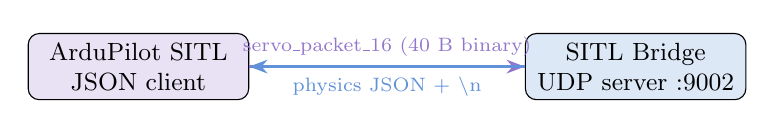
\begin{tikzpicture}[>=Stealth, node distance=3.5cm]
  \node[draw, rounded corners, fill=ardu!15, minimum width=2.8cm, minimum height=0.8cm, align=center, font=\small]
    (ap) {ArduPilot SITL\\JSON client};
  \node[draw, rounded corners, fill=simblue!15, minimum width=2.8cm, minimum height=0.8cm, align=center,
        font=\small, right=of ap] (bridge2) {SITL Bridge\\UDP server :9002};
  \draw[->, thick, ardu!70] (ap) -- node[above, font=\scriptsize]{servo\_packet\_16 (40 B binary)} (bridge2);
  \draw[->, thick, simblue!70] (bridge2) -- node[below, font=\scriptsize]{physics JSON + \textbackslash n} (ap);
\end{tikzpicture}
\end{center}

The physics JSON sent each step:

\begin{lstlisting}[language=Python, caption={Physics state dict sent to ArduPilot}, label={lst:physics}]
{
  "timestamp": 1234.5,
  "imu": {
    "gyro":       [0.0, 0.0, yaw_rate],
    "accel_body": [sf_bx, sf_by, sf_bz]   # specific force (m/s^2)
  },
  "attitude":  [0.0, 0.0, yaw_rad],
  "velocity":  [vn, ve, vd],              # required=true in SIM_JSON.h
  "rng_1":     agl_m,
  "battery":   {"voltage": 12.6, "current": 5.0}
  # "position" intentionally ABSENT -- AnyLoc provides it via MAVLink instead
}
\end{lstlisting}

\paragraph{Key design point.} The \texttt{"position"} field is a GPS substitute in
ArduPilot's EKF3.  It is deliberately omitted to enforce GPS-denied operation.
\texttt{"velocity"} (\texttt{required=true}) stays to prevent ArduPilot from rejecting the
packet.

\subsubsection*{EKF3 Configuration (\texttt{no\_gps.parm})}

\begin{lstlisting}[caption={SITL parameter file for GPS-denied operation}]
GPS_TYPE        0   # disable GPS sensor
EK3_SRC1_POSXY  6   # horizontal position: ExternalNav (AnyLoc)
EK3_SRC1_VELXY  0   # no horizontal velocity source
EK3_SRC1_POSZ   1   # altitude from barometer
EK3_SRC1_YAW    1   # yaw from compass
VISO_TYPE       1   # enable MAVLink ExternalNav processing
\end{lstlisting}

\subsubsection*{MAVLink Controller (\texttt{mavlink\_ctrl.py})}

\texttt{MAVLinkCtrl} is a non-blocking pymavlink wrapper that:
\begin{itemize}
  \item maintains the latest \texttt{HEARTBEAT}, \texttt{HIGHRES\_IMU}, \texttt{ATTITUDE},
        \texttt{LOCAL\_POSITION\_NED}, and \texttt{EKF\_STATUS\_REPORT} in memory;
  \item sends \texttt{VISION\_POSITION\_ESTIMATE} (AnyLoc position \ensuremath{\to} EKF3);
  \item exposes \texttt{arm()}, \texttt{takeoff()}, \texttt{set\_position\_ned()} for 6b-iv.
\end{itemize}

\subsubsection*{EKF Status Flags}

\begin{table}[h]
\centering
\caption{EKF\_STATUS\_REPORT flag bits (ArduPilot EKF3)}
\begin{tabular}{@{}lrll@{}}
\toprule
\textbf{Constant} & \textbf{Bit} & \textbf{Hex} & \textbf{Meaning}\\
\midrule
\texttt{EKF\_ATTITUDE}        & 0  & 0x0001 & Attitude valid\\
\texttt{EKF\_VEL\_HORIZ}      & 1  & 0x0002 & Horizontal velocity valid\\
\texttt{EKF\_POS\_HORIZ\_REL} & 3  & 0x0008 & Relative horizontal position valid\\
\texttt{EKF\_POS\_HORIZ\_ABS} & 4  & 0x0010 & Absolute position valid (vision fused) $\leftarrow$ \textit{target}\\
\texttt{EKF\_PRED\_POS\_HORIZ\_ABS} & 9 & 0x0200 & Vision estimate accepted\\
\texttt{EKF\_UNINITIALIZED}   & 10 & 0x0400 & EKF not yet initialised (normal at startup)\\
\bottomrule
\end{tabular}
\end{table}

\subsubsection*{Vision Bridge (\texttt{run\_vision.py})}

Reads \texttt{anyloc/latest\_estimate.json} and converts to NED relative to SITL home:

\[
  N = (\phi_\text{est} - \phi_\text{home}) \cdot 111{,}320, \quad
  E = (\lambda_\text{est} - \lambda_\text{home}) \cdot 111{,}320 \cdot \cos\phi_\text{home}, \quad
  D = -(\text{alt} - \text{alt}_\text{home})
\]

Sends \texttt{VISION\_POSITION\_ESTIMATE} at 5 Hz on TCP port 5763 (separate from the
monitor on 5762, since each TCP port accepts one client).  Covariance: 20 m horizontal
std ($\approx$AnyLoc anchor error), 5 m vertical, 0.3 rad yaw.

Confirmed result: EKF flags reach \texttt{ATT,VEL\_H,VEL\_V,POS\_REL,POS\_ABS,ALT,PRED\_ABS}
--- full fusion achieved (Milestone 6b-iii).

\subsubsection*{Stub Bridge (\texttt{stub\_bridge.py})}

A kinematic hover simulator driven by ArduPilot's PWM outputs.  Allows MAVLink
testing without Isaac Sim running:

\begin{itemize}
  \item Integrates thrust from mean motor PWM into vertical velocity and altitude.
  \item Horizontal position fixed at scene origin (drone hovers in place).
  \item Runs at 100 Hz; sends the same physics JSON as the real bridge.
\end{itemize}

% ─────────────────────────────────────────────────────────────────────────────
\section{Repository Layout}
\label{sec:layout}
% ─────────────────────────────────────────────────────────────────────────────

\begin{lstlisting}[caption={Project directory tree},label={lst:tree}]
no_GPS_drone_project/
+-- instructions/
|   +-- project_plan.md       # module status, design decisions, milestones
|   +-- history.md            # session-by-session change log
+-- simulator/
|   +-- cesium_scene.py       # Isaac Sim scene: terrain + drone + camera + bridge
|   +-- drone_frames/         # live output: latest.jpg + latest_meta.json
|   +-- run_chiayi.sh         # launch script
+-- anyloc/
|   +-- build_database.py     # build VLAD database from NLSC orthophoto (once)
|   +-- localizer.py          # AnyLocLocalizer (DINOv2 + VLAD + FAISS)
|   +-- vo_refiner.py         # VORefiner (LK optical flow)
|   +-- run_localizer.py      # live dual postview + writes latest_estimate.json
|   +-- database/             # 2821-entry VLAD database (49152-dim, 50 m grid)
+-- detection/
|   +-- detector.py           # YOLODetector (auto class-map)
|   +-- run_detector.py       # live annotated postview
|   +-- label_writer.py       # nadir projection for synthetic labels
|   +-- collect_training_data.py  # Isaac Sim synthetic data collector
|   +-- prepare_dataset.py    # VisDrone + remap + merge synth
|   +-- finetune.py           # YOLOv8 top-down fine-tuning
+-- yolov8l_visdrone.pt       # active model (VisDrone 10-class)
+-- control/
|   +-- sitl_bridge.py        # UDP :9002 server --- binary servo in, JSON physics out
|   +-- stub_bridge.py        # kinematic hover stub for MAVLink testing
|   +-- mavlink_ctrl.py       # MAVLinkCtrl + EKF constants + vision + cmds
|   +-- run_mavlink.py        # live terminal EKF monitor (port 5762)
|   +-- run_vision.py         # AnyLoc -> VISION_POSITION_ESTIMATE (port 5763)
|   +-- no_gps.parm           # SITL: GPS_TYPE=0, EK3_SRC1_POSXY=6, VISO_TYPE=1
|   +-- imu_reader.py         # HIGHRES_IMU reader [TODO 6c]
|   +-- imu_fusion.py         # anchor validator + VO gate [TODO 6d]
+-- third_party/
|   +-- ardupilot/            # ArduPilot source; binary: build/sitl/bin/arducopter
+-- main.py                   # top-level orchestrator [TODO]
\end{lstlisting}

% ─────────────────────────────────────────────────────────────────────────────
\section{Running the System}
\label{sec:quickstart}
% ─────────────────────────────────────────────────────────────────────────────

\subsection*{Requirements}

\begin{itemize}
  \item NVIDIA GPU (RTX 2080 Ti or better, 8 GB+ VRAM)
  \item NVIDIA driver 520+; Ubuntu 22.04 / 24.04
  \item conda env \texttt{isaac\_sim\_test} (Python 3.12, Isaac Sim 6.0.0)
  \item Cesium ion account (token embedded in \texttt{cesium\_scene.py})
  \item X11 display (\texttt{DISPLAY=:2} or virtual framebuffer)
  \item System Python packages: \texttt{pexpect mavproxy pymavlink future}
\end{itemize}

\subsection*{Build ArduPilot SITL (one-time)}

\begin{lstlisting}[language=bash, numbers=none]
cd third_party/ardupilot
git submodule update --init --depth=1 --recursive   # ~5 min
python3 waf configure --board sitl
python3 waf copter                                   # ~2 min
cd ../..
\end{lstlisting}

\subsection*{Launch Order (5 terminals)}

\begin{lstlisting}[language=bash, numbers=none, caption={Terminal 1 --- ArduPilot SITL}]
python3 third_party/ardupilot/Tools/autotest/sim_vehicle.py \
    -v ArduCopter --model=JSON --no-rebuild --console --map \
    -l 23.450868,120.286135,46,0 \
    --add-param-file=control/no_gps.parm \
    --out tcp:localhost:5763
\end{lstlisting}

\begin{lstlisting}[language=bash, numbers=none, caption={Terminal 2 --- Isaac Sim (or stub)}]
# Full simulation:
cd simulator && ./run_chiayi.sh

# Or lightweight stub (no Isaac Sim needed):
python3 control/stub_bridge.py
\end{lstlisting}

\begin{lstlisting}[language=bash, numbers=none, caption={Terminal 3 --- AnyLoc localizer}]
DISPLAY=:2 conda run -n isaac_sim_test python anyloc/run_localizer.py
\end{lstlisting}

\begin{lstlisting}[language=bash, numbers=none, caption={Terminal 4 --- Vision bridge (AnyLoc -> EKF3)}]
python3 control/run_vision.py
\end{lstlisting}

\begin{lstlisting}[language=bash, numbers=none, caption={Terminal 5 --- MAVLink monitor}]
python3 control/run_mavlink.py
\end{lstlisting}

\subsection*{Expected EKF Progression}

\begin{lstlisting}[numbers=none]
TIME     ROLLdeg   PCHdeg    YAWdeg      N m      E m      D m    EKF flags
------  ------  ------  ------  ------   ------   ------  ---------
  5.0    0.00    0.00    0.00    0.00     0.00    -5.00  0x0400 UNINIT
 10.0    0.01   -0.02    0.00    0.00     0.00    -5.00  0x0001 ATT
 40.0    0.01   -0.02   90.00    0.12     0.05    -9.87  0x003f ATT,VEL,POS_ABS
\end{lstlisting}

\texttt{POS\_ABS} (bit 4) confirms that EKF3 has accepted the AnyLoc vision position.
Flight commands will now work.

\subsection*{Rebuild the AnyLoc Database}

Only needed after the scene or camera FOV changes:

\begin{lstlisting}[language=bash, numbers=none]
conda run -n isaac_sim_test python anyloc/build_database.py --rebuild
\end{lstlisting}

% ─────────────────────────────────────────────────────────────────────────────
\section{Milestones}
\label{sec:milestones}
% ─────────────────────────────────────────────────────────────────────────────

\begin{longtable}{@{}clll@{}}
\toprule
\textbf{\#} & \textbf{Milestone} & \textbf{Status}\\
\midrule
\endhead
1 & Isaac Sim scene: Cesium terrain + NLSC imagery + OSM buildings & Done\\
2 & Virtual drone + nadir camera publishing frames & Done\\
3 & AnyLoc map database built from simulated views & Done\\
4 & AnyLoc localisation + dual postview on simulated frames & Done\\
5 & YOLO detection working on simulated frames & Done\\
5a & Switch to VisDrone-trained YOLOv8l; auto class-map in detector & Done\\
5b & Top-down fine-tuning pipeline (VisDrone + synthetic data) & Ready to run\\
6a & ArduPilot SITL + Isaac Sim JSON bridge (IMU + baro) & Done\\
6b-i & pymavlink connection to ArduPilot MAVLink output & Done\\
6b-ii & Disable GPS; strip position from JSON bridge (IMU+baro only) & Done\\
6b-iii & AnyLoc $\to$ ArduPilot EKF3 via \texttt{VISION\_POSITION\_ESTIMATE} & Done\\
6b-iv & Flight commands via \texttt{SET\_POSITION\_TARGET} (replaces keyboard) & TODO\\
6c & \texttt{HIGHRES\_IMU} from ArduPilot $\to$ localisation pipeline & TODO\\
6d & IMU fusion: AnyLoc anchor validator + VO quality gate & TODO\\
7 & Full pipeline integrated in simulation & TODO\\
8 & Deploy to real hardware & TODO\\
\bottomrule
\end{longtable}

% ─────────────────────────────────────────────────────────────────────────────
\section{Key Design Decisions}
\label{sec:decisions}
% ─────────────────────────────────────────────────────────────────────────────

\paragraph{ArduPilot before custom IMU fusion.}
On real hardware, IMU data arrives as MAVLink \texttt{HIGHRES\_IMU} messages.  Building against
the MAVLink interface now means \textit{zero code changes} at hardware deployment.
ArduPilot's own sensor models (bias drift, noise, temperature) are more realistic than
analytical position derivatives.

\paragraph{No numpy --- torch tensors throughout.}
The \texttt{isaac\_sim\_test} conda environment has a dual numpy conflict
(pip numpy 2.x vs.\ conda numpy 1.26.4 from faiss-cpu).  All VLAD pipeline operations use
torch tensors; numpy is only touched at C-level FAISS call sites where the ABI is compatible.

\paragraph{Geo-constrained AnyLoc search.}
Unconstrained VLAD retrieval can jump to visually similar but geographically distant tiles
(e.g.\ two similar road intersections 800 m apart).  The 200 m window reduces the candidate
set from 2,821 to $\approx$50 entries, making wrong-tile matches geometrically impossible.

\paragraph{Vision position, not bridge position.}
The JSON bridge's \texttt{"position"} field is a GPS substitute in ArduPilot's EKF3.
Sending it would give the EKF ground truth, not AnyLoc estimates.  It is intentionally
absent; AnyLoc position arrives via \texttt{VISION\_POSITION\_ESTIMATE} instead
--- the same mechanism as Intel RealSense T265 or OptiTrack on real hardware.

\paragraph{Two MAVLink TCP ports.}
Each TCP port accepts exactly one client.  The monitor (\texttt{run\_mavlink.py}) uses port 5762;
the vision bridge (\texttt{run\_vision.py}) uses port 5763 (opened with \texttt{--out tcp:localhost:5763}).

% ─────────────────────────────────────────────────────────────────────────────
\section{Competition Readiness}
\label{sec:competition}
% ─────────────────────────────────────────────────────────────────────────────

The competition (2nd UAV Defense Challenge) requires GPS-denied autonomous UAV operation
with multi-target vehicle detection and geo-location.

\begin{table}[h]
\centering
\caption{Competition requirement gap analysis}
\begin{tabular}{@{}p{4cm}p{4cm}p{4.5cm}@{}}
\toprule
\textbf{Requirement} & \textbf{Current state} & \textbf{Gap}\\
\midrule
GPS-denied navigation & AnyLoc + VO (done) & Integrate ArduPilot autonomous flight\\
Civilian vehicle detection & \texttt{yolov8l\_visdrone.pt} (done) & Verify car-roof logo detection\\
Military vehicle detection & Not in VisDrone classes & Collect aerial training data; fine-tune\\
Oil drums detection & Not in current model & Collect data; fine-tune\\
Amphibious APC detection & Not in current model & Collect data; fine-tune\\
Geo-location accuracy ($\leq$50 m) & 15--20 m anchor error & Meets requirement ($\varepsilon_i = 10$, full score)\\
GCS live display & matplotlib windows & Verify HDMI output to judges\\
Return-to-home & ArduPilot RTL (stub) & Wire up after Milestone 6b-iv\\
\bottomrule
\end{tabular}
\end{table}

The localisation accuracy of $\approx15$--20 m satisfies the competition's tightest scoring
bracket ($\leq$50 m \ensuremath{\to} full 10 position points per target).

% ─────────────────────────────────────────────────────────────────────────────
\section*{Acknowledgements}
% ─────────────────────────────────────────────────────────────────────────────

\begin{itemize}
  \item \textbf{AnyLoc} --- ``AnyLoc: Towards Universal Visual Place Recognition'', IRAL 2024.
        \url{https://github.com/AnyLoc/AnyLoc}
  \item \textbf{YOLOv8} --- Ultralytics. \url{https://github.com/ultralytics/ultralytics}
  \item \textbf{ArduPilot} --- Open-source autopilot. \url{https://ardupilot.org}
  \item \textbf{Isaac Sim 6.0} --- NVIDIA. \url{https://developer.nvidia.com/isaac-sim}
  \item \textbf{Taiwan NLSC PHOTO2} --- National Land Surveying and Mapping Center, National Land Surveying and Mapping Center, Taiwan.
\end{itemize}

\end{document}
